% standalone document border convention: {left bottom right top}
\documentclass[varwidth=406pt,border={0pt, -4pt, 0pt, -10pt}]{standalone}
\usepackage[force]{feynmp-auto}		    
\usepackage{amsmath}
\usepackage{graphicx}
\usepackage{simpler-wick}

% Path to Figure directory
\graphicspath{{/home/daniel/latex/hfm_paper/7_diagrams/FeynmanDiagram.jl/diagrams/}}

\begin{document}
\begin{flalign*}
	G_{12} \hspace*{0.5ex}&=\hspace*{0.5ex} \langle \mathcal{T} \psi_2 {\psi^\dagger_1} \rangle_0 
	\hspace*{0.5ex}-\hspace*{0.5ex}
	V_{34} \langle \mathcal{T} \wick[offset=3ex]{
		\c1 {\psi_2}
		\c1 {\psi^\dagger_3} \c1 {\psi^\dagger_4}
		\c1 {\psi_4} \c1 {\psi_3}
		\c1 {\psi^\dagger_1}
	} \rangle_0
	\hspace*{0.5ex}-\hspace*{0.5ex}
	V_{34} \langle \mathcal{T} \wick[offset=3ex]{
		\c1 {\psi_2}
		\c2 {\psi^\dagger_3} \c1 {\psi^\dagger_4}
		\c2 {\psi_4} \c1 {\psi_3}
		\c1 {\psi^\dagger_1}
	} \rangle_0 \\[1ex]
	&\hspace*{2.5ex}+\hspace*{0.5ex}
	V_{34} V_{56} \langle \mathcal{T} \wick[offset=3ex]{
		\c1 {\psi_2}
		\c5 {\psi^\dagger_3} \c4 {\psi^\dagger_4}
		\c3 {\psi_4} \c2 {\psi_3}
		\c1 {\psi^\dagger_5} \c3 {\psi^\dagger_6}
		\c4 {\psi_6} \c5 {\psi_5}
		\c2 {\psi^\dagger_1}
	} \rangle_0
	\hspace*{0.5ex}+\hspace*{0.5ex}
	V_{34} V_{56} \langle \mathcal{T} \wick[offset=3ex]{
		\c2 {\psi_2}
		\c5 {\psi^\dagger_3} \c4 {\psi^\dagger_4}
		\c1 {\psi_4} \c3 {\psi_3}
		\c1 {\psi^\dagger_5} \c2 {\psi^\dagger_6}
		\c4 {\psi_6} \c5 {\psi_5}
		\c3 {\psi^\dagger_1}
		} \rangle_0
	\hspace*{0.5ex}+\hspace*{0.5ex}\cdots \\[1ex]
	&=\hspace*{0.5ex} g_{12} 
	\hspace*{0.5ex}+\hspace*{0.5ex}
	(-1)^2 V_{34} \, g_{13} \, g_{32} \, g_{44}
	\hspace*{0.5ex}+\hspace*{0.5ex}
	(-1) V_{34} \, g_{13} \, g_{34} \, g_{42} \\[1ex]
	&\hspace*{2.5ex}+\hspace*{0.5ex}
	(-1)^3 V_{34} V_{56} \, g_{13} \, g_{35} \, g_{52} \, g_{46} \, g_{64}
	\hspace*{0.5ex}+\hspace*{0.5ex}
	(-1)^2 V_{34} V_{56} \, g_{13} \, g_{35} \, g_{54} \, g_{46} \, g_{62} 
	\hspace*{0.5ex}+\hspace*{0.5ex}\cdots \\
	&=\hspace*{-0.5ex}
	\raisebox{1.75ex}{
		\scalebox{0.75}{$
				\begin{gathered}
					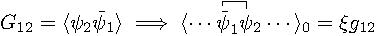
\includegraphics{green/green0.pdf}
				\end{gathered}
			$}
	}
	\hspace*{-0.5ex}+\hspace*{-0.5ex}
	\raisebox{1.75ex}{
		\scalebox{0.75}{$
				\begin{gathered}
					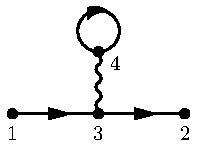
\includegraphics{green/green1a.pdf}
				\end{gathered}
			$}
	}
	\hspace*{-0.5ex}+\hspace*{-0.5ex}
	\raisebox{1.75ex}{
		\scalebox{0.75}{$
				\begin{gathered}
					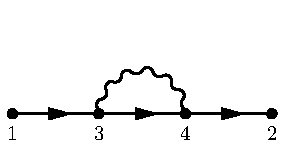
\includegraphics{green/green1b.pdf}
				\end{gathered}
			$}
	} \\
	&\hspace*{2.5ex}+\hspace*{-0.5ex}
	\raisebox{1.75ex}{
		\scalebox{0.75}{$
				\begin{gathered}
					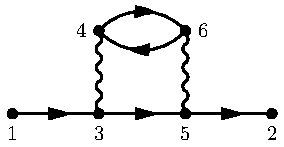
\includegraphics{green/green2a.pdf}
				\end{gathered}
			$}
	}
	\hspace*{-0.5ex}+\hspace*{-0.5ex}
	\raisebox{1.75ex}{
		\scalebox{0.75}{$
				\begin{gathered}
					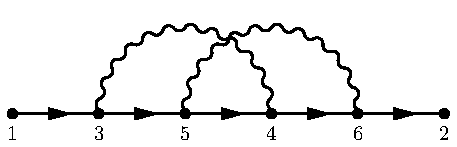
\includegraphics{green/green2b.pdf}
				\end{gathered}
			$}
	}
	\hspace*{-0.5ex}+\hspace*{0.5ex} \cdots
\end{flalign*}
\end{document}
